%%This is a very basic article template.
%%There is just one section and two subsections.
\documentclass{article}

\usepackage{amsmath}
\usepackage{amsfonts}
\usepackage{parskip}
\usepackage{cleveref}
\usepackage{xcolor} 
\usepackage{graphicx}
\usepackage{tikz}
\usepackage{pgfplots}
\usetikzlibrary{plotmarks}
\setlength{\parskip}{0.2cm}

\title{TTIC 31230 Project Report}

\author{Hao Jiang}
\begin{document}

\maketitle

\section{Introduction}
I am interested in LSTM RNN architecture related questions and would 
like to address this kind of problem in the project. More specifically,
I want to understand how multi-layer RNNs can improve the performance
comparing to single-layer RNN.

A typical LSTM Neural Network structure is demonstrated in \Cref{fig:lstm}. It
comprised of multiple LSTM (Long short-memory) cells. All the cells have the same 
structure and share the same parameter sets. The $i$-th cell takes input 
$X_i$ from external source, it also carries two internal states, namely 
the carry state $c_i$, denoted by the top horizontal line, and hidden state
$h_i$, denoted by the bottom horizontal line. The cell makes computations 
based on the input and states, then emits the updated states $c_{i+1}$ and 
$h_{i+1}$ to next cell. The output of each cell is computed based on the 
hidden state $h_{i+1}$. 
 
\begin{figure}
\centering
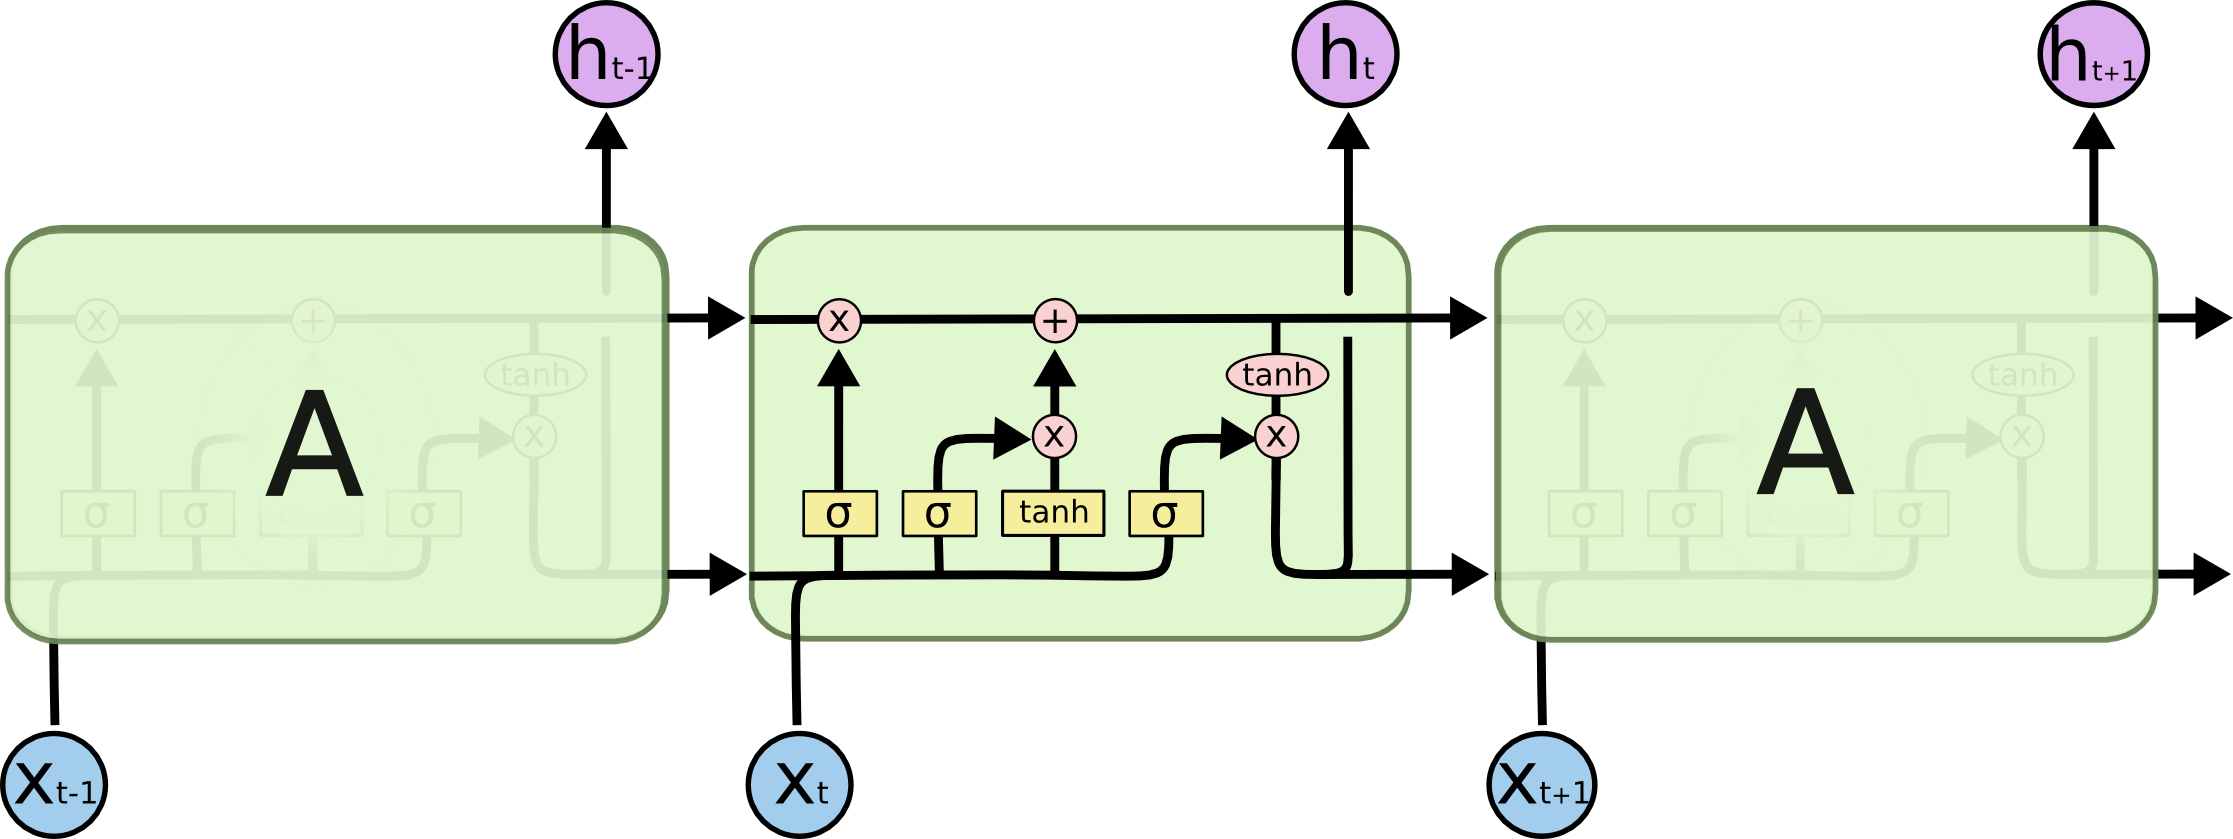
\includegraphics[scale=0.7]{lstm.png} 
\caption{Long Short Term Memory RNN}
\label{fig:lstm}
\end{figure} 

RNN has gained significant improvement in sequence data processing mostly
due to its specialized architecture. The carry state connecting LSTM cells
serves as the memory of RNN. In each step, the memory can be forgotten, or enhanced
based on both the new input and the hidden state. The output of each cell also
depends on the carry state of current cell.

A natural extension of RNN is the multi-layer RNN. A single layer RNN only
extends the network in 1-d dimension, while multi-layer RNN allows the network
to expand on 2-d dimensions. \Cref{fig:mllstm} shows a 2-layer LSTM network. The
upper layer RNN maintains its own carry state, and will take the hidden state
from the layer below it as input. Intuitively, this structure allows the upper
layer to get summarized information from the lower layer and generate a more 
general memory state. The more layer is added to the structure, the more
general information can be captured by the RNN at the top layer.

\begin{figure}
\centering
\includegraphics[scale=0.7]{mllstm.png} 
\caption{Multi-Layer LSTM}
\label{fig:mllstm}
\end{figure} 

\section{Experiment}

Theoretically, adding more layers can be beneficiary to reducing the loss. However,
more layers almost certainly cost more time to train. Is the reduced loss worthy
for the extra training time? In additional, increasing the hidden dimension size
should also reduce loss at the cost of training time. Which method is more efficient?

To answer these questions, I conducted a series of experiments that varies both
the number of layers and the size of hidden dimensions. The experiment
parameters are listed in \Cref{tab:param}. The table shows how many epoches are 
executed for each layer and hidden dimension combination.

\renewcommand{\arraystretch}{1.2}
\begin{table}
\centering
\begin{tabular}{c|c|c|c|c}
\textbf{Layer\textbackslash HD} & 200 & 300 & 400 & 600\\
\hline
2 & 90& 90& 90& 30 \\
\hline
3 & 90& 90& 90& 30 \\
\hline
4 & 90& 90& 90& - \\
\end{tabular}
\caption{Experiment Parameter}
\label{tab:param}
\end{table}

All experiments are conducted on Dell PowerEdge R630 equipped with 2 Intel Xeon
CPU E5-2670 v3 @ 2.30GHz, 128GB memory running Ubuntu 16.04. The software 
environment is Numpy 1.11.2 running on Python 3.5.2 with the latest Intel MKL
library. In this experiment I use 7 machines with a total training time of 
over 400 hours. In all subsequent experiments, we leave step size to be 0.5 and
decay rate to be 0.9.

We first evaluate the relationship between number of layers / size of hidden
dimensions and training time. This is demonstrated in \Cref{fig:time} and
\Cref{tab:time}. It can be noticed that as expected, the training time is
proportional to the product of number of layers and hidden dimension.

\begin{figure}
\centering
\begin{tikzpicture}
\begin{axis}[xlabel=Epoches, ylabel=Training Time (mins),
legend entries={HD 200 Layer 2, HD 200 Layer 3, HD 200 Layer 4,
HD 300 Layer 2, HD 300 Layer 3, HD 300 Layer 4, HD 400 Layer 2,
HD 400 Layer 3, HD 400 Layer 4},
legend style={at={(10cm,1.2cm)},anchor=south east}]
\addplot[red, mark=o,mark size=1.5] table[x=ep,y=l2] {data/hd_200_time};
\addplot[blue, mark=x, mark size=1.5] table[x=ep,y=l3] {data/hd_200_time};
\addplot[black,mark=+, mark size=1.5] table[x=ep,y=l4] {data/hd_200_time};
\addplot[red,mark=square,mark size=1.5] table[x=ep,y=l2] {data/hd_300_time};
\addplot[blue,mark=triangle,mark size=1.5] table[x=ep,y=l3] {data/hd_300_time};
\addplot[black,mark=diamond,mark size=1.5] table[x=ep,y=l4] {data/hd_300_time};
\addplot[red,mark=pentagon,mark size=1.5] table[x=ep,y=l2] {data/hd_400_time};
\addplot[blue,mark=triangle*,mark size=1.5] table[x=ep,y=l3] {data/hd_400_time};
\addplot[black,mark=diamond*,mark size=1.5] table[x=ep,y=l4] {data/hd_400_time};
\end{axis}
\end{tikzpicture}
\caption{Training time}
\label{fig:time}
\end{figure}

\begin{table}
\centering
\begin{tabular}{c|c|c|c|c}
\textbf{Layer\textbackslash HD} & 200 & 300 & 400 & 600\\ 
\hline
2 & 16.250& 25.223& 36.142& - \\
\hline
3 & 24.108& 38.072& 54.319& - \\
\hline 
4 & 32.186& 51.019& 72.489& - \\
\end{tabular}
\caption{Average Training Time Per Epoch (min)}
\label{tab:time}
\end{table}

We then explore how much accuracy improvement can be brought by increasing
number of layers. \Cref{tab:hd200loss}, \Cref{tab:hd300loss} and
\Cref{tab:hd400loss} demonstrates the result when the size of hidden layer
is 200, 300 and 400 respectively.


\begin{figure}
\centering
\begin{tikzpicture}
\begin{axis}[xlabel={Epoches}, ylabel={Average Loss},
legend entries={2 Layers, 3 Layers, 4 Layers}]
\addplot[red, mark=o,mark size=1] table[x=ep,y=l2] {data/hd_200_loss};
\addplot[blue, mark=x,mark size=1] table[x=ep,y=l3] {data/hd_200_loss};
\addplot[black, mark=+,mark size=1] table[x=ep,y=l4] {data/hd_200_loss};
\end{axis}
\end{tikzpicture}
\caption{Loss for different number of Layers for hidden dimension 200}
\label{tab:hd200loss}
\end{figure}

\begin{figure}
\centering
\begin{tikzpicture}
\begin{axis}[xlabel={Epoches}, ylabel={Average Loss},
legend entries={2 Layers, 3 Layers, 4 Layers}]
\addplot[red, mark=o,mark size=1] table[x=ep,y=l2] {data/hd_300_loss};
\addplot[blue, mark=x,mark size=1] table[x=ep,y=l3] {data/hd_300_loss};
\addplot[black, mark=+,mark size=1] table[x=ep,y=l4] {data/hd_300_loss};
\end{axis}
\end{tikzpicture}
\caption{Loss for different number of Layers for hidden dimension 300}
\label{tab:hd300loss}
\end{figure}

\begin{figure}
\centering
\begin{tikzpicture}
\begin{axis}[xlabel={Epoches}, ylabel={Average Loss},
legend entries={2 Layers, 3 Layers, 4 Layers}]
\addplot[red, mark=o,mark size=1] table[x=ep,y=l2] {data/hd_400_loss};
\addplot[blue, mark=x,mark size=1] table[x=ep,y=l3] {data/hd_400_loss};
\addplot[black, mark=+,mark size=1] table[x=ep,y=l4] {data/hd_400_loss};
\end{axis}
\end{tikzpicture}
\caption{Loss for different number of Layers for hidden dimension 400}
\label{tab:hd400loss}
\end{figure}
 
The result is anti-intuitive that although significant amount of training time
is consumed for more layers and larger hidden dimensions, the gain is not
proportional to it. In fact, when look at all the graphs, we can notice that
more layers always takes more training epoches to converge, while finally
the loss converge to the same level with negligible difference. In fact in all
hidden dimension sizes, 3 layers always yield 2$\sim$3\% better result than the
other two options at the end of our training process. 

An explanation to this scenario is that more layers and larger hidden
dimensions all make the model taking longer time to converge. Just as 3 layers
excels 2 layers with 90 epoches, 4 layers may perform best if we increase the
training epoches to a larger number. However, in my opinion, the gain from
additional layers / hidden dimensions is not significant enough to compensate
the additional training time.

We also would like to understand how increasing hidden dimension size would help
improving efficiency. In \Cref{fig:hdl2}, \Cref{fig:hdl3} and \Cref{fig:hdl4},
we demonstrate how loss will vary with epoches when hidden dimension increases.
Not surprisingly, increase hidden dimension does help, but to a very limited
extent. In all cases, we again only get 1$\sim$2\% improvement when doubling the
hidden dimension from 200 to 400.
\begin{figure}
\centering
\begin{tikzpicture}
\begin{axis}[xlabel={Epoches}, ylabel={Average Loss},
legend entries={HD 200, HD 300, HD 400}]
\addplot[red, mark=o,mark size=1] table[x=ep,y=l2] {data/hd_200_loss};
\addplot[blue, mark=x,mark size=1] table[x=ep,y=l2] {data/hd_300_loss};
\addplot[black, mark=+,mark size=1] table[x=ep,y=l2] {data/hd_400_loss};
\end{axis}
\end{tikzpicture}
\caption{Loss of different hidden dimensions for 2 Layer}
\label{fig:hdl2}
\end{figure}

\begin{figure}
\centering
\begin{tikzpicture}
\begin{axis}[xlabel={Epoches}, ylabel={Average Loss},
legend entries={HD 200, HD 300, HD 400}]
\addplot[red, mark=o,mark size=1] table[x=ep,y=l3] {data/hd_200_loss};
\addplot[blue, mark=x,mark size=1] table[x=ep,y=l3] {data/hd_300_loss};
\addplot[black, mark=+,mark size=1] table[x=ep,y=l3] {data/hd_400_loss};
\end{axis}
\end{tikzpicture}
\caption{Loss of different hidden dimensions for 3 Layer}
\label{fig:hdl3}
\end{figure}

\begin{figure}
\centering
\begin{tikzpicture}
\begin{axis}[xlabel={Epoches}, ylabel={Average Loss},
legend entries={HD 200, HD 300, HD 400}]
\addplot[red, mark=o,mark size=1] table[x=ep,y=l4] {data/hd_200_loss};
\addplot[blue, mark=x,mark size=1] table[x=ep,y=l4] {data/hd_300_loss};
\addplot[black, mark=+,mark size=1] table[x=ep,y=l4] {data/hd_400_loss};
\end{axis}
\end{tikzpicture}
\caption{Loss of different hidden dimensions for 4 Layer}
\label{fig:hdl4}
\end{figure}

Finally we demonstrate how perplexity changes when we vary hidden dimensions and
number of layers. The result is shown in \Cref{fig:perp}. It can be seen that
in every case, the result converges to almost the same level. 
\begin{figure}
\centering
\begin{tikzpicture}
\begin{axis}[xlabel={Epoches}, ylabel={Perplexity},
legend entries={HD 200 Layer 2, HD 300 Layer 2, HD 400 Layer 2,
HD 200 Layer 3, HD 300 Layer 3, HD 400 Layer 3,
HD 200 Layer 4, HD 300 Layer 4, HD 400 Layer 4}]
\addplot[red, mark=o,mark size=1] table[x=ep,y=l2] {data/hd_200_perp};
\addplot[blue, mark=o,mark size=1] table[x=ep,y=l2] {data/hd_300_perp};
\addplot[black, mark=o,mark size=1] table[x=ep,y=l2] {data/hd_400_perp};
\addplot[red, mark=x,mark size=1] table[x=ep,y=l3] {data/hd_200_perp};
\addplot[blue, mark=x,mark size=1] table[x=ep,y=l3] {data/hd_300_perp};
\addplot[black, mark=x,mark size=1] table[x=ep,y=l3] {data/hd_400_perp};
\addplot[red, mark=+,mark size=1] table[x=ep,y=l4] {data/hd_200_perp};
\addplot[blue, mark=+,mark size=1] table[x=ep,y=l4] {data/hd_300_perp};
\addplot[black, mark=+,mark size=1] table[x=ep,y=l4] {data/hd_400_perp};
\end{axis}
\end{tikzpicture}
\caption{Perplexity for different layers and hidden dimensions}
\label{fig:perp}
\end{figure}
\section{Future Work}
This preliminary result is somewhat frustrating as it shows that simply adding
more layers or increasing hidden dimension size help only little in improving
system performance. In addition, as we can see from the experiment result,
the predict text is still far from perferct. For example, as we have seen in
class, a well-trained LSTM could simulate Shakespear's work, while the best
result from my training process can only generate sentences like ``the company
said it will be a \textless unk\textgreater of the \textless unk\textgreater
\ldots'' My future work will be focus on how an architecture change can help
LSTM to generate meaningful sentences.
\section{Conclusion}
In this project, I explore how different combination of hidden dimension size
and number of layers can affect the performance of LSTM RNN. Surprisingly,
increasing hidden dimension size and add more layers do not have obvious effect
in reducing loss, while do consumes significant more amount of training time.
Although this conclusion need to be further verified by further increasing
training epoches, using larger dimension and more layers, this preliminary
result shows that increasing the size of hidden dimensions does not always help.

\end{document}

